
\def\k{k}
%\def\kluc{kľúč}
\def\put{$\mathop{insert}(\k)$}
\def\find{$\mathop{find}(\k)$}
\def\delete{$\mathop{delete}(\k)$}
\def\trie{trie}
\def\uz{{\tt\$}}

\section{Písmenkový strom}
\emph{Abeceda} je množina \emph{znakov}. \emph{Slovo} je postupnosť znakov 
z danej abecedy. \emph{Písmenkový strom} je \emph{zakorenený strom}, v ktorom 
každá hrana obsahuje práve jeden znak z abecedy alebo \emph{ukončovací znak}. 
\emph{Ukončovací znak} je ľubovoľný, dopredu dohodnutý symbol, ktorý sa 
v abecede nenachádza. My používame ako abecedu veľké znaky anglickej 
abecedy a ukončovací znak značíme dolárom (\uz).



\paragraph{Popis.}
Strom obsahuje slová nazývané \emph{kľúče}. Po prejdení cesty 
z koreňa do vrcholu s \emph{ukončovacím znakom} prečítame kľúč.%
\footnote{Na hranách $h_1, h_2, \ldots, h_n$ sú znaky $z_1, z_2, \ldots, 
z_{n-1}, $\uz, ktoré po zreťazení utvoria slovo $z_1z_2\ldots{z_{n-1}}$.} 
Teda, oproti binárnym vyhľadávacím stromom je hlavný rozdiel v tom, že 
kľúče nie sú uložené vo vrcholoch, ale samotná poloha v strome určuje kľúč. 
Písmenkový strom sa podobne ako binárny vyhľadávací strom využíva ako 
\emph{asociatívne pole (slovník)}, takže poskytuje tieto tri operácie:
\begin{itemize}
\item $\mathop{\mathbf{insert}}(\k)$ -- pridá do stromu kľúč $\k$;
\item $\mathop{\mathbf{find}}(\k)$ -- zistí, či sa v strom kľúč $\k$ nachádza;
\item $\mathop{\mathbf{delete}}(\k)$ -- odstráni zo stromu kľúč $\k$ a 
prípadne vyrieši zmeny v strome.
\end{itemize}
Všetky operácie začínajú v koreni a ku kľúču pridávajú ukončovací znak, 
teda pracujú s reťazcom $\k\emph{\$}$. 

Operácia \put\ vloží do stromu vstupný reťazec tak, že z reťazca berie znaky 
a prechádza po príslučných hranách. Ak hrana so znakom neexistuje pridá ju. 

Operácia \find\ sa spustí z koreňa podľa postupnosti znakov. Ak hrana, 
po ktorej sa má spustiť neexistuje, daný kľúč sa v strome nenachádza. 
Ak prečítame celý vstupný reťazec, daný kľúč sa v strome nachádza.

Operácia \delete\ najprv pomocou operácie \find\ zistí umiestnenie kľúča. 
Ak sa kľúč v strome nachádza, algoritmus odstráni hranu s ukončovacím 
symbolom a vrchol, ktorý bol na nej zavesený. V tomto štádiu sa nám môže 
stať, že v strome ostane takzvaná \emph{mŕtva vetva} -- nie je ukončená 
ukončovacím znakom. Pre fungovanie stromu to nevadí, všetky operácie by 
prebiehali správne, ale takto štruktúra zaberá zbytočne veľa miesta. 
Preto je dobré túto mŕtvu vetvu odstrániť.

\begin{figure}
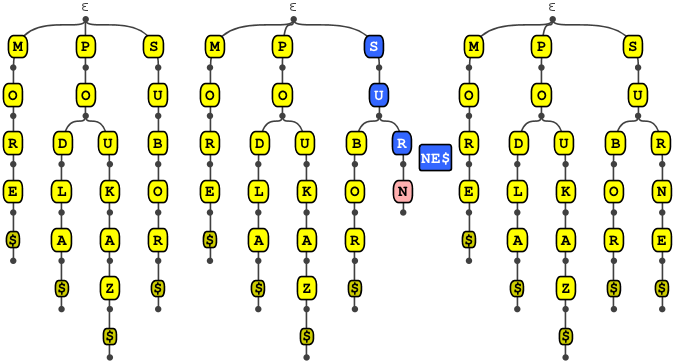
\includegraphics[width=\columnwidth]{obrazky/trieinsertsmall.png}
\caption{\emph{Operácia \put.} Vo vizualizácií naznačujeme, kade sa 
presunieme.} 
\label{img:trieinsert} 
\end{figure}

\begin{figure}
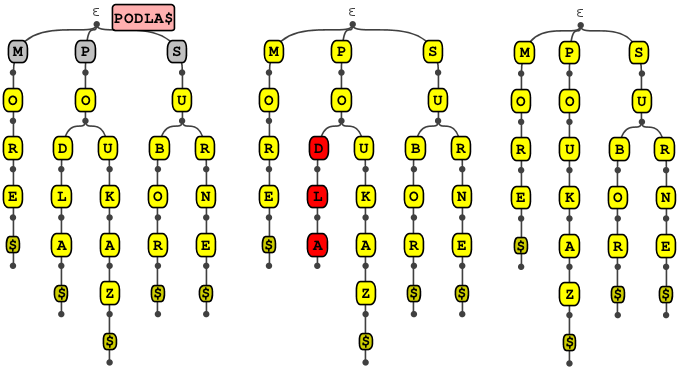
\includegraphics[width=\columnwidth]{obrazky/triedeletesmall.png}
\caption{\emph{Operácia \delete.} \emph{Mŕtva vetva} je vyznačená červenou.
%Najprv zistíme, či je kľúč v strome, 
%potom ho zmažeme a potom zmažeme mŕtvu vetvu, ktorá je vyznačená 
%červenou farbou.
} 
\label{img:triedelete} 
\end{figure}

\paragraph{Použitie.}
Vďaka tomu, že písmenkový strom udržiava spoločné \emph{prefixy} kľúčov sa 
nazýva aj \emph{prefixový strom}.
Prvý krát popísal písmenkový strom \citet{fredkin}, ktorý používal názov 
\emph{trie memory}, keďže išlo o spôsob udržiavania dát v pamäti. Pojem 
\emph{trie}\footnote{Z anglického re\emph{trie}val -- získanie.} 
sa rozšíril a používa sa celosvetovo.
%používal operácie 
%$\mathop{storage}$ (\put), $\mathop{retrieval}$ (\find) 
%a $\mathop{deletion}$ (\delete) a dátovú štruktúru nazýval \emph{trie 
%memory}, keďže išlo naozaj o spôsob uloženia dát v pamäti.

O niečo neskôr \citet{knuth} uviedol vo svojej knihe ako príklad na 
písmenkový strom vreckový slovník. V tom istom diele uviedol aj možnosť 
komprimovania vetiev a možnosť prerobenia $m$-árneho \trie\ na binárny. 
\citet{knuth} však ukázal len komprimovanie koncov vetiev. Písmenkový 
strom, v ktorom každý vrchol, ktorého otec má len jedného syna 
je zlúčený s otcom\footnote{Na hranách teda nie sú znaky, ale slová.}, 
popísal \citet{patricia} a zaviedol pre ňho pojem \emph{PATRICIA}. 
Pre túto dátovú štruktúru sa používa aj pojem \emph{radix tree (radix trie)}. 

Dátovú štruktúru podobnú \emph{hashovacej tabuľke} a písmenkovému stromu 
popísal vo svojej dizertačnej práci \citet{liang} a nazval ju \emph{packed 
trie}. Oproti obyčajnému písmenkovému stromu výrazne šetrila miesto. 
V práci ju využil na vytvorenie vzorcov pre slabikovanie slov.

Písmenkové stromy sa podobajú na \emph{konečné automaty}. 
Vznikli rôzne modifikácie stromov na automaty, ktorých hlavnou výhodou je, 
že v komprimovanej podobe spájajú nielen predpony, ale aj prípony slov 
a teda v slovách ľudských jazykov výrazne znižujú pamäťový priestor potrebný 
na uchovanie dátovej štruktúry \citep{scrabble,ca}. 

Priamočiare je použitie písmenkového stromu na utriedenie poľa slov. 
Všetky slová sa pridajú do stromu a potom sa spraví \emph{preorderový prechod} 
stromu. Túto myšlienku spracovali \citet{burstsort1} a veľmi výrazne zrýchlil 
triedenie dlhých zoznamov slov. Neskôr tento algoritmus vylepšili 
\citet{burstsort2}. Kvôli tomu, ako algoritmus pracuje, 
sa nazýva \emph{burstsort}.

Špeciálnym použitím písmenkového stromu je vytvorenie stromu zo všetkých 
prípon slova. Táto dátova štruktúra sa nazýva \emph{sufixový strom} a dá sa 
mo\-di\-fi\-ko\-vať na udržiavanie viacerých slov. Tieto štruktúry majú 
veľmi veľa praktických využití \citep{gusfield}. 

%Friker, neobzeraj baby a pracuj! 
%Nejaké citovateľné práce o trie?

